\begin{figure}[htbp]
	\centering
    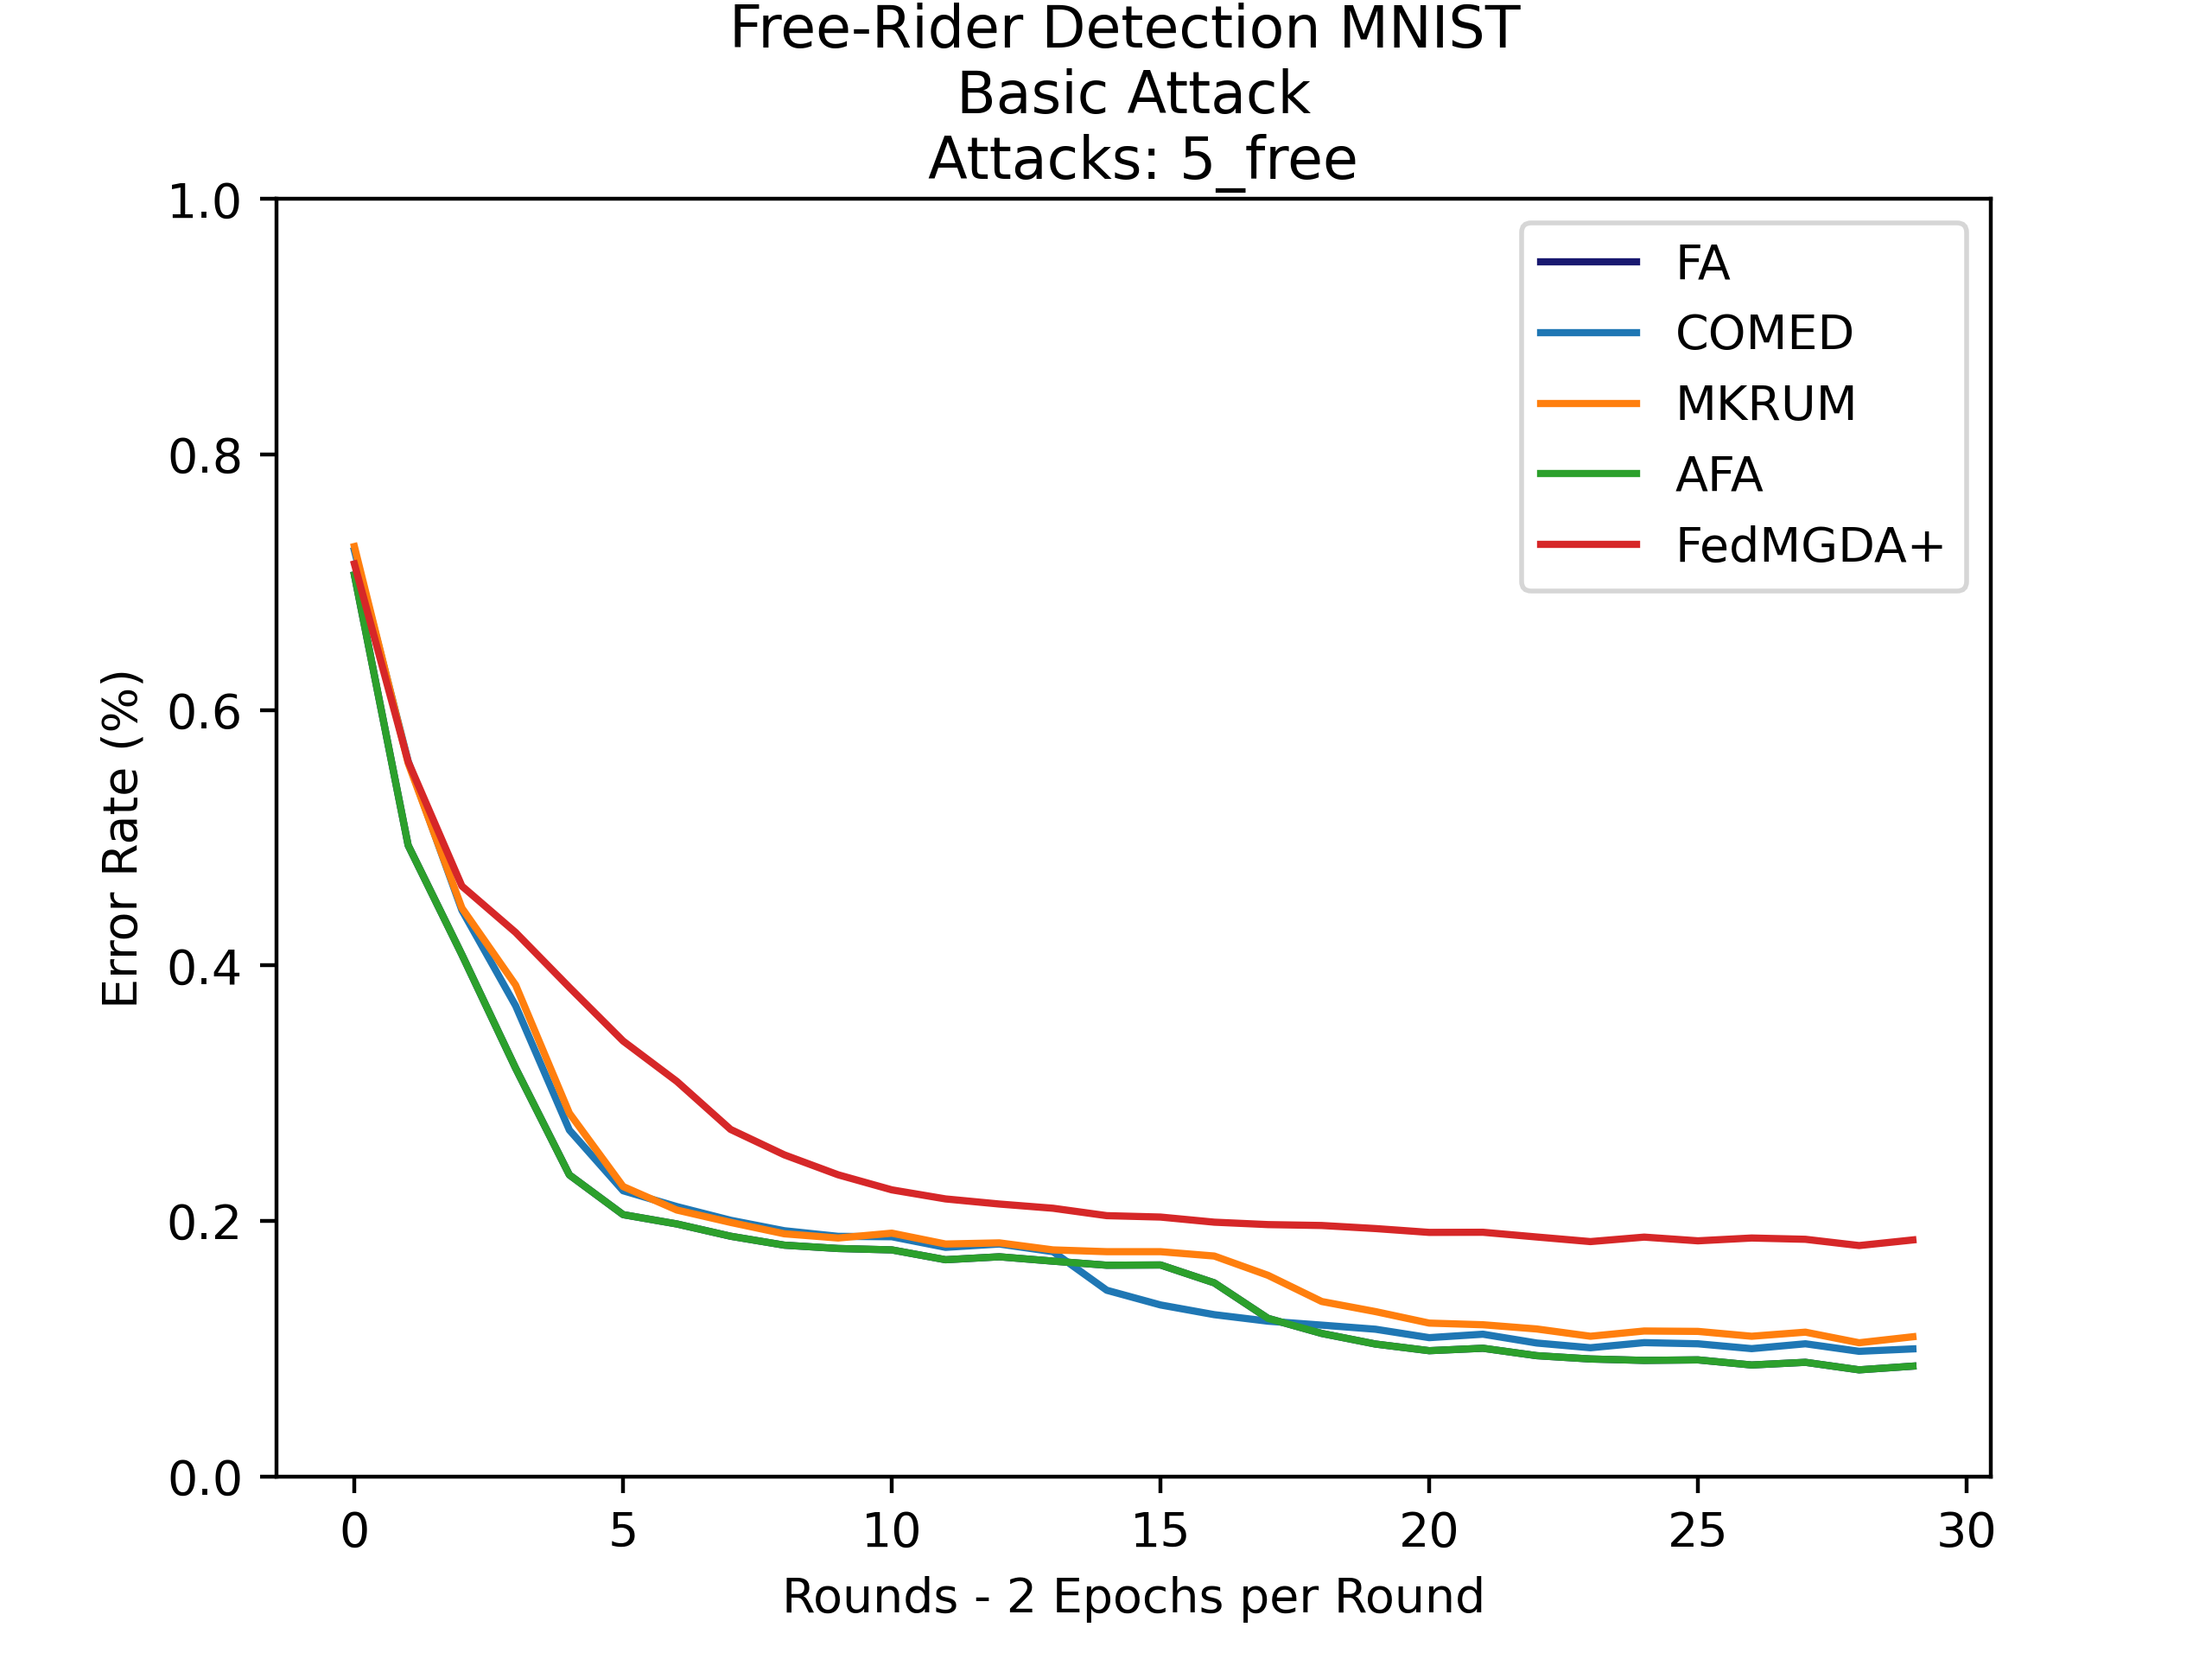
\includegraphics[scale=0.5]{free_riders/graphs/basic5.png}
	\caption{Basic Attack with 5 Free-Riders - Basically No Damage Done}
	\label{fig:5free}
\end{figure}

\begin{figure}[htbp]
	\centering
    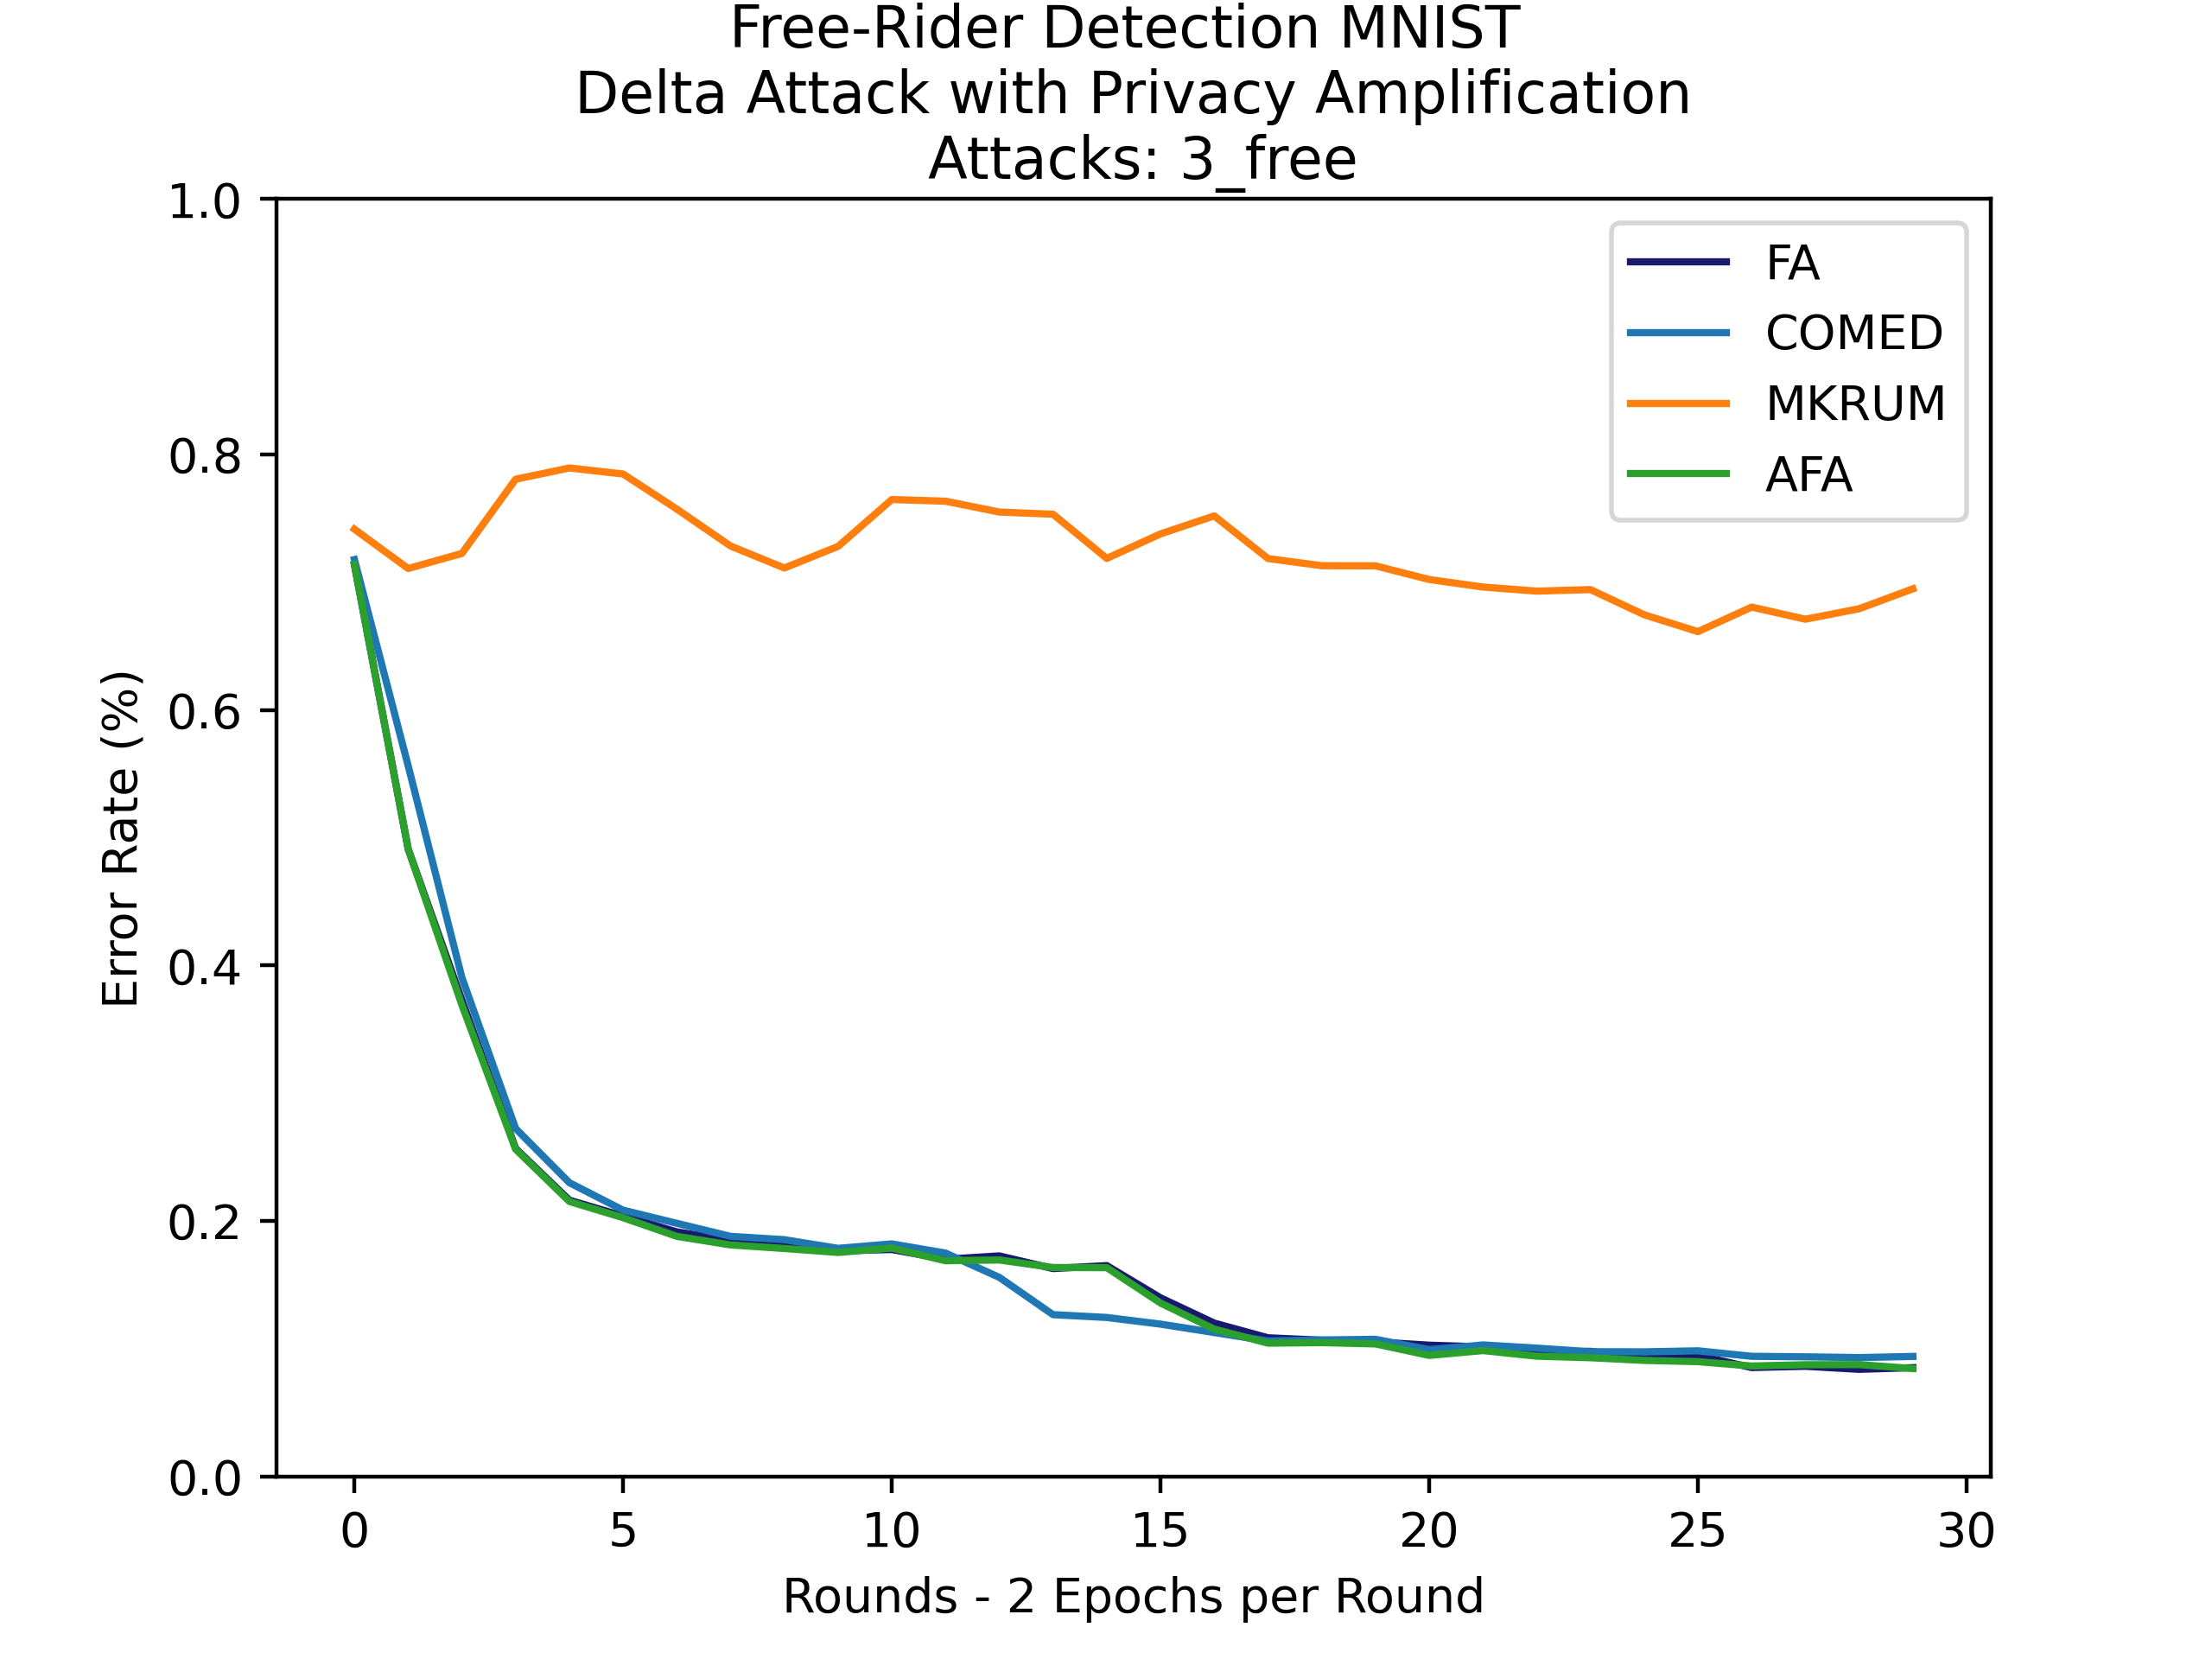
\includegraphics[scale=0.5]{free_riders/graphs/mkrum_suffer.png}
	\caption{MKRUM Suffering with Only 3 Free-Riding Clients under Privacy Amplification with a Delta-Weight Attack}
	\label{fig:mkrum_suf}
\end{figure}

\begin{figure}[htbp]
	\centering
    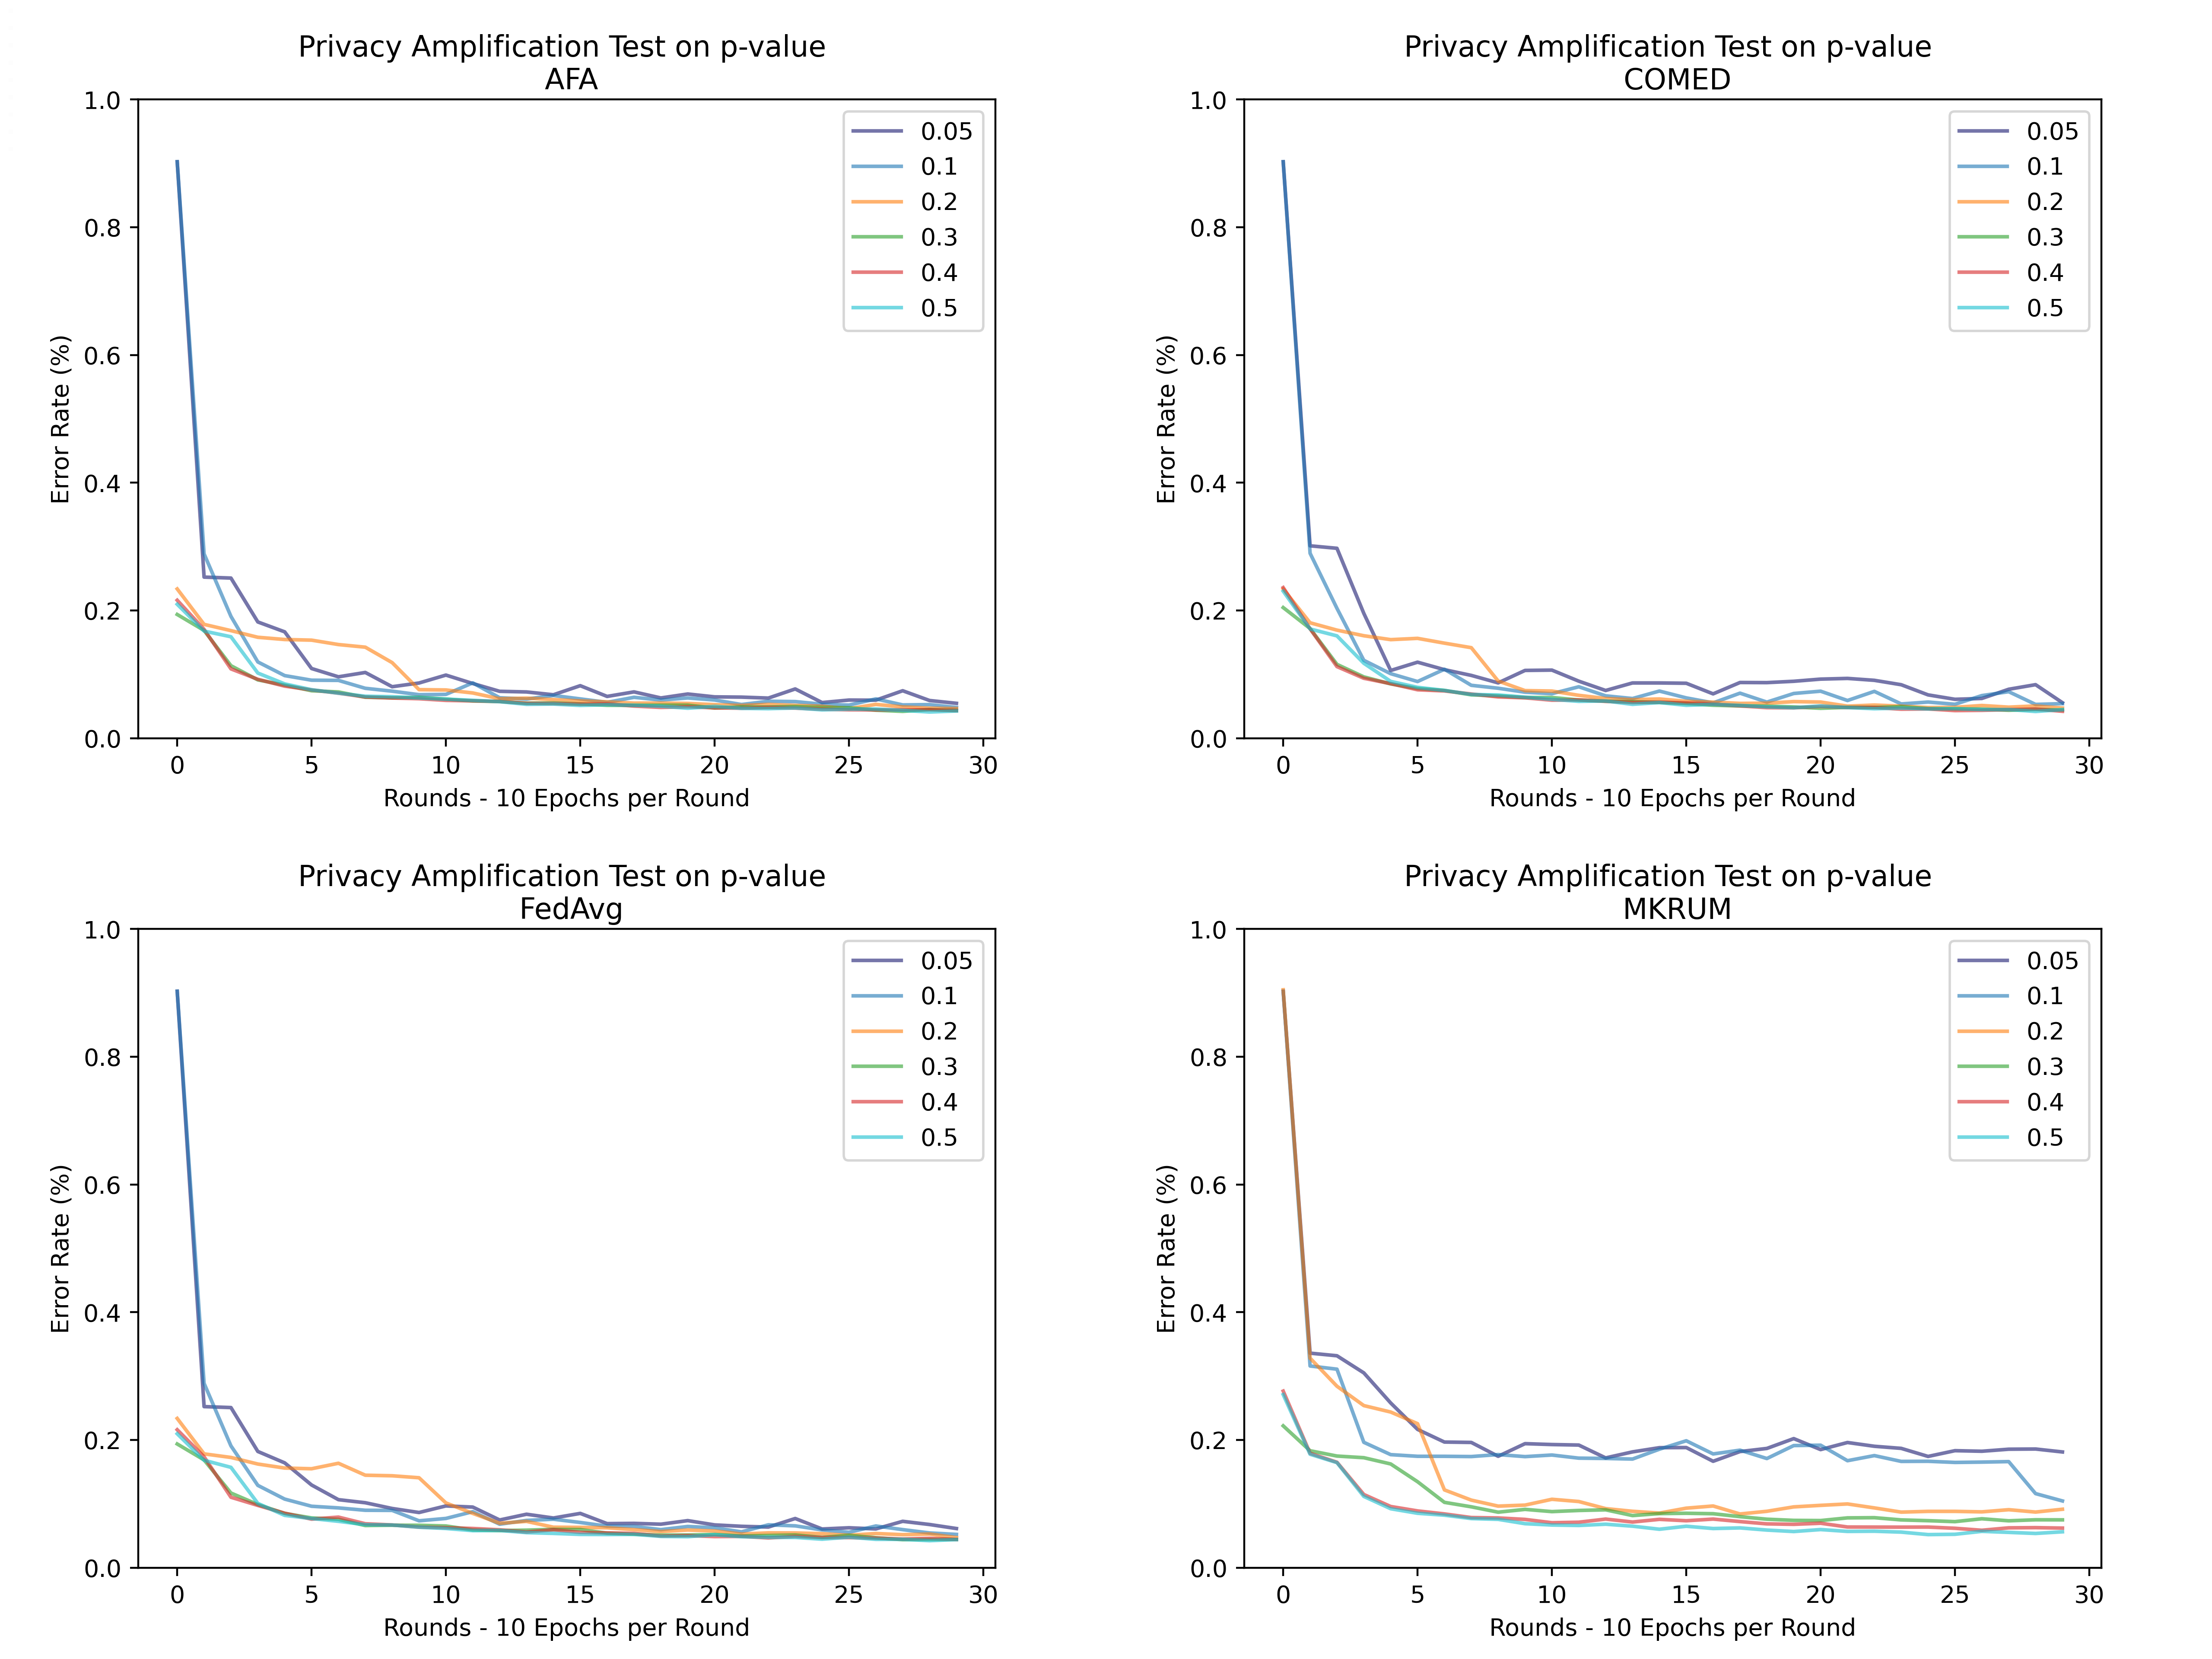
\includegraphics[scale=0.07]{free_riders/graphs/p_test.png}
	\caption{Privacy Amplification with Uniform Sampling with p-Thresholds - 10 epochs}
	\label{fig:p_test}
\end{figure}

\begin{figure}[htbp]
	\centering
    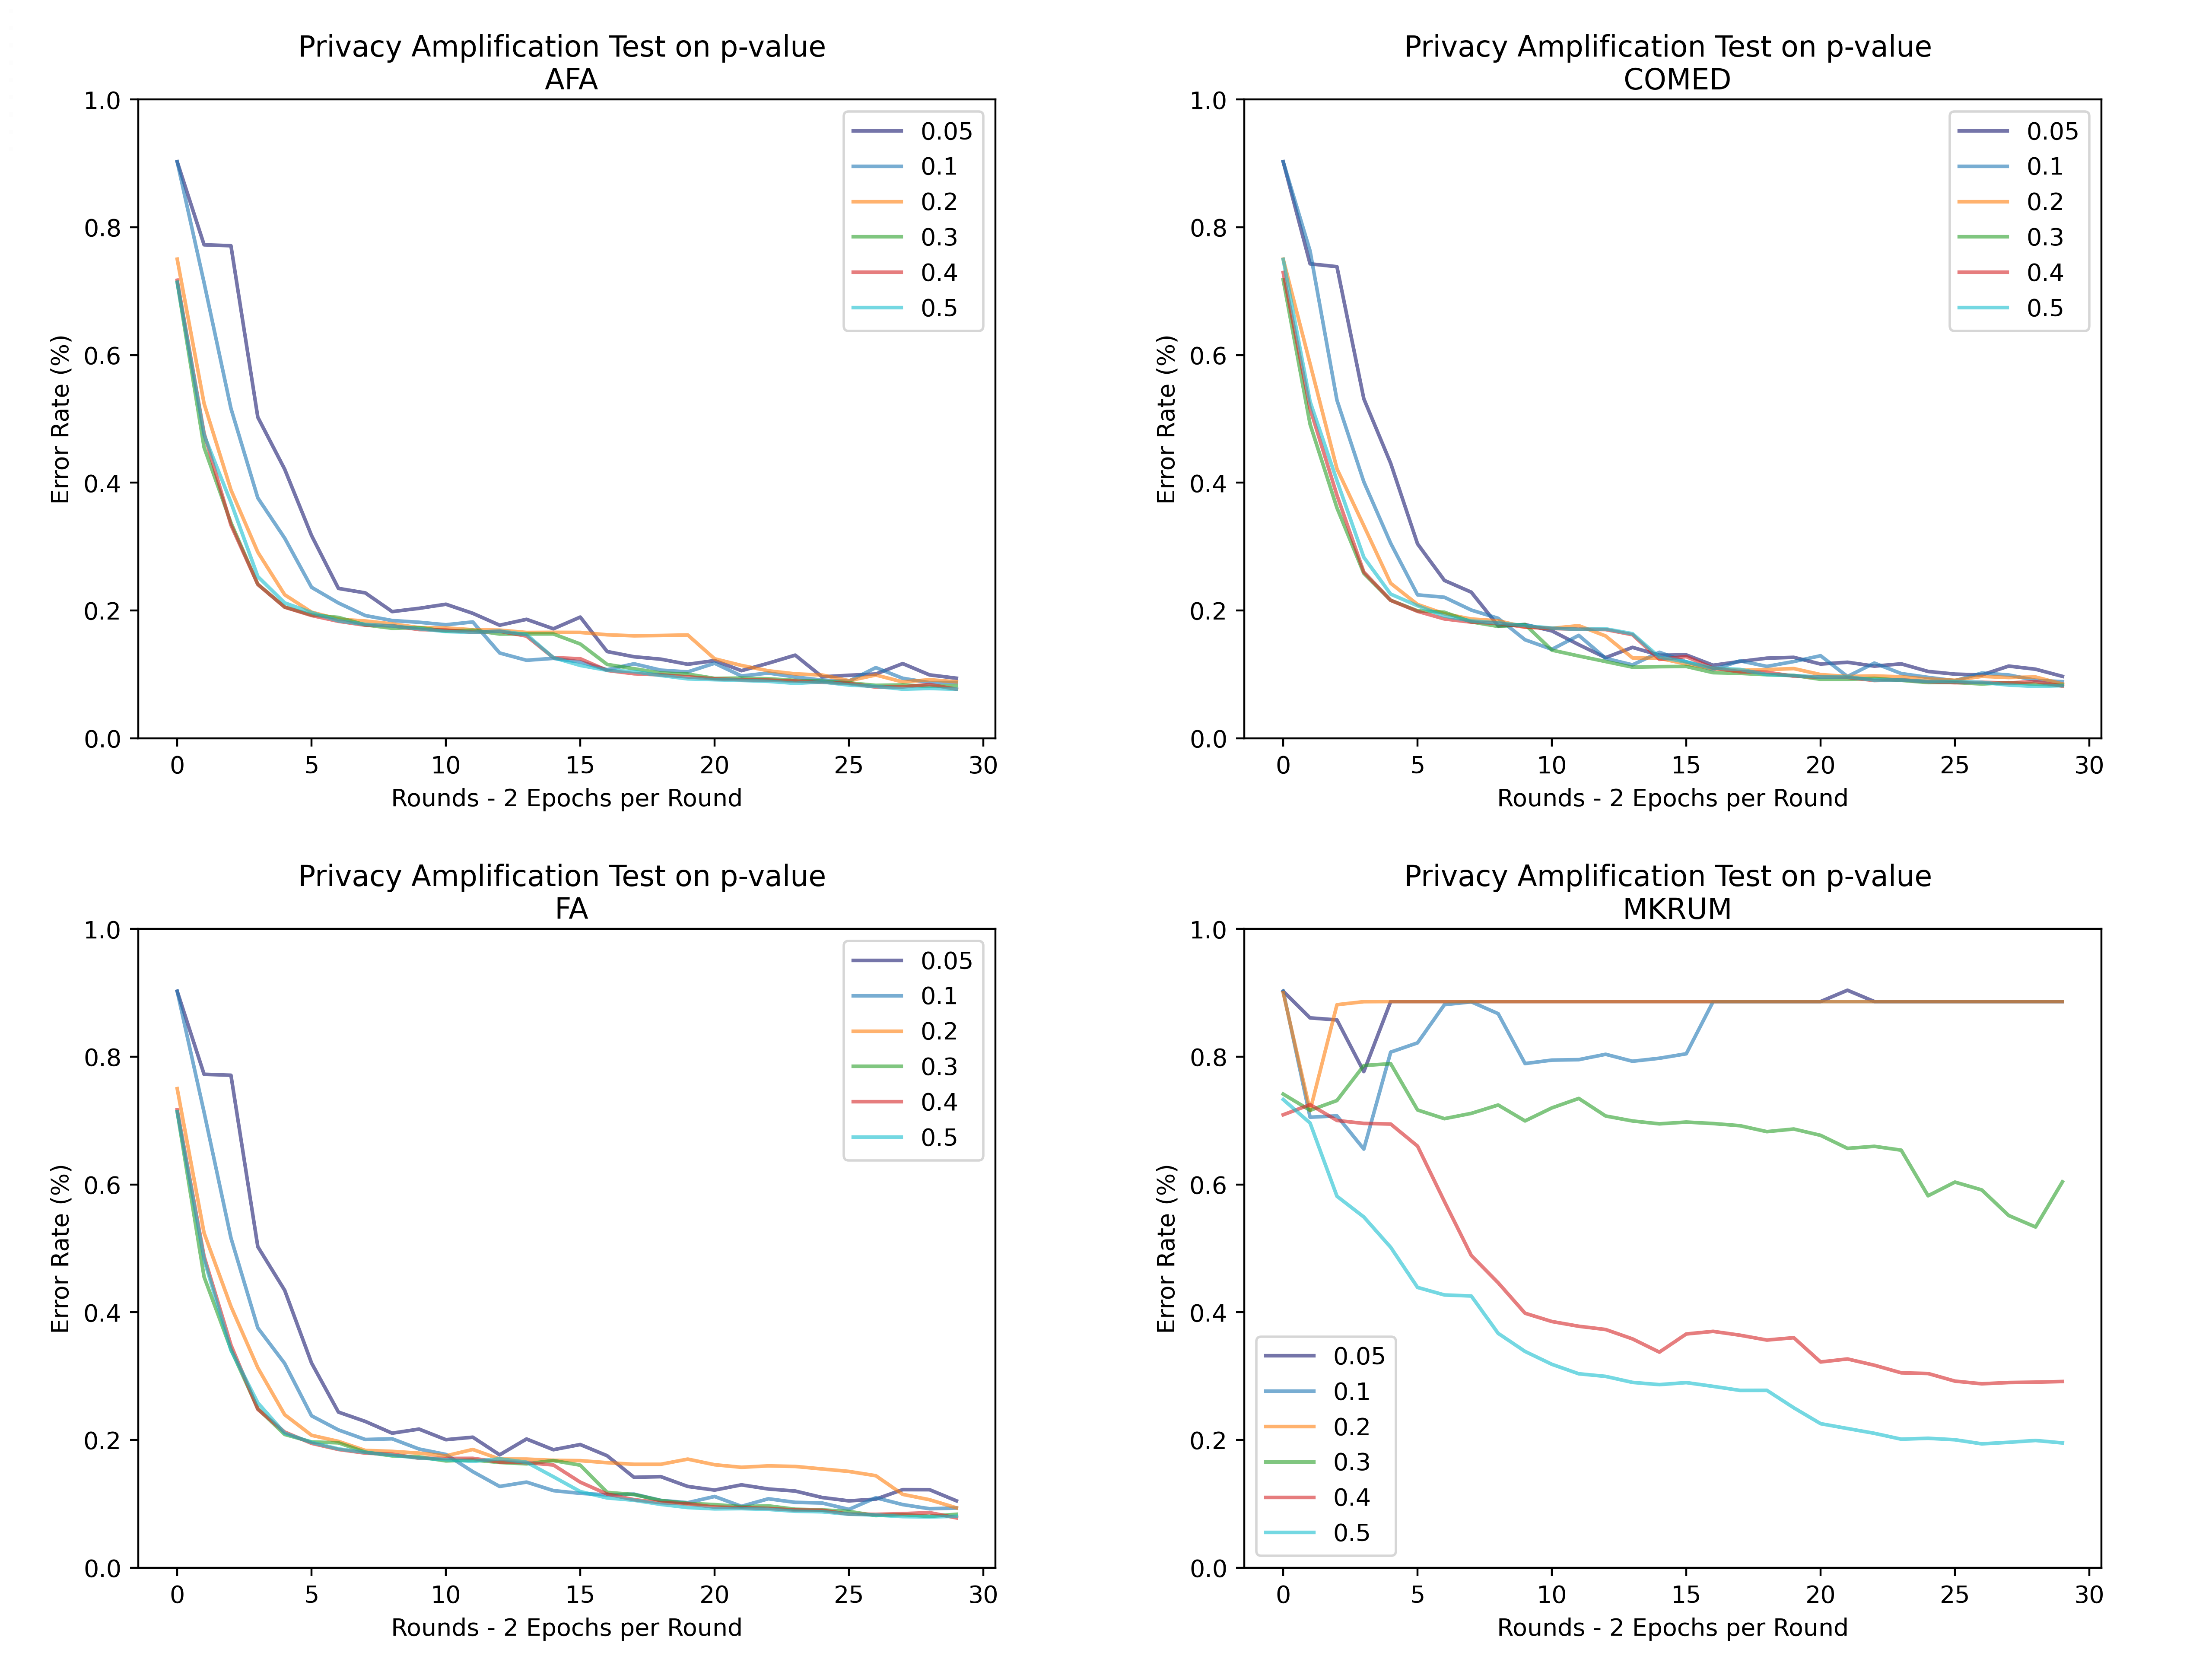
\includegraphics[scale=0.07]{free_riders/graphs/p_test_2.png}
	\caption{Privacy Amplification with Uniform Sampling with p-Thresholds - 2 epochs}
	\label{fig:p_test_2}
\end{figure}

\begin{figure}[htbp]
	\centering
    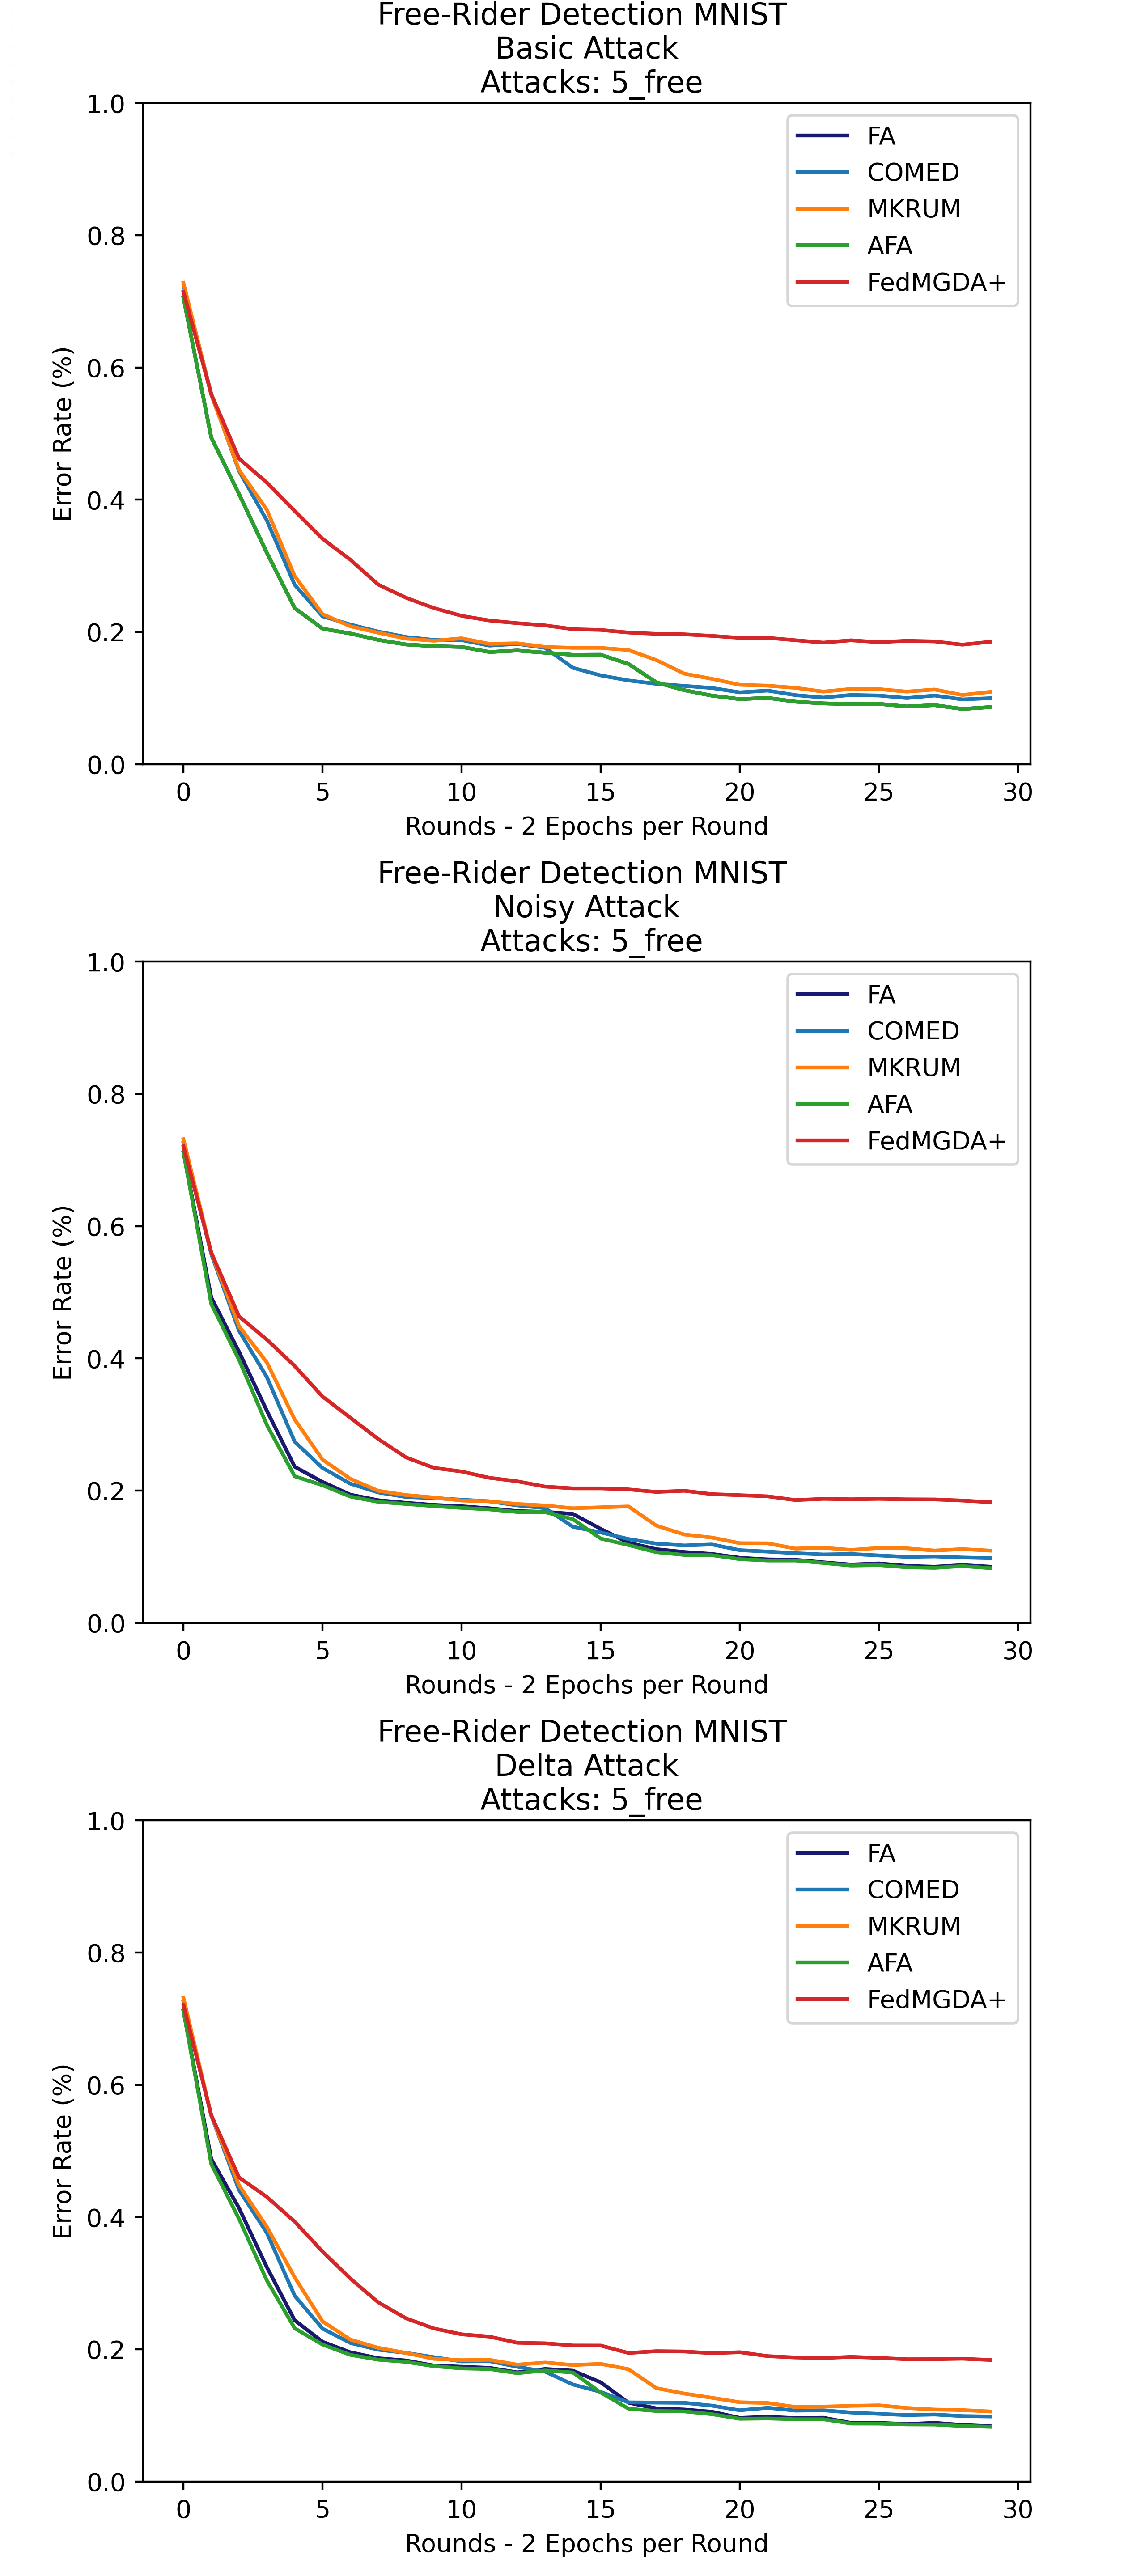
\includegraphics[scale=0.1]{free_riders/graphs/no_dmg.png}
	\caption{Minimal Performance Degradation with 5 Free-Riders}
	\label{fig:no_dmg}
\end{figure}

\begin{figure}[htbp]
	\centering
    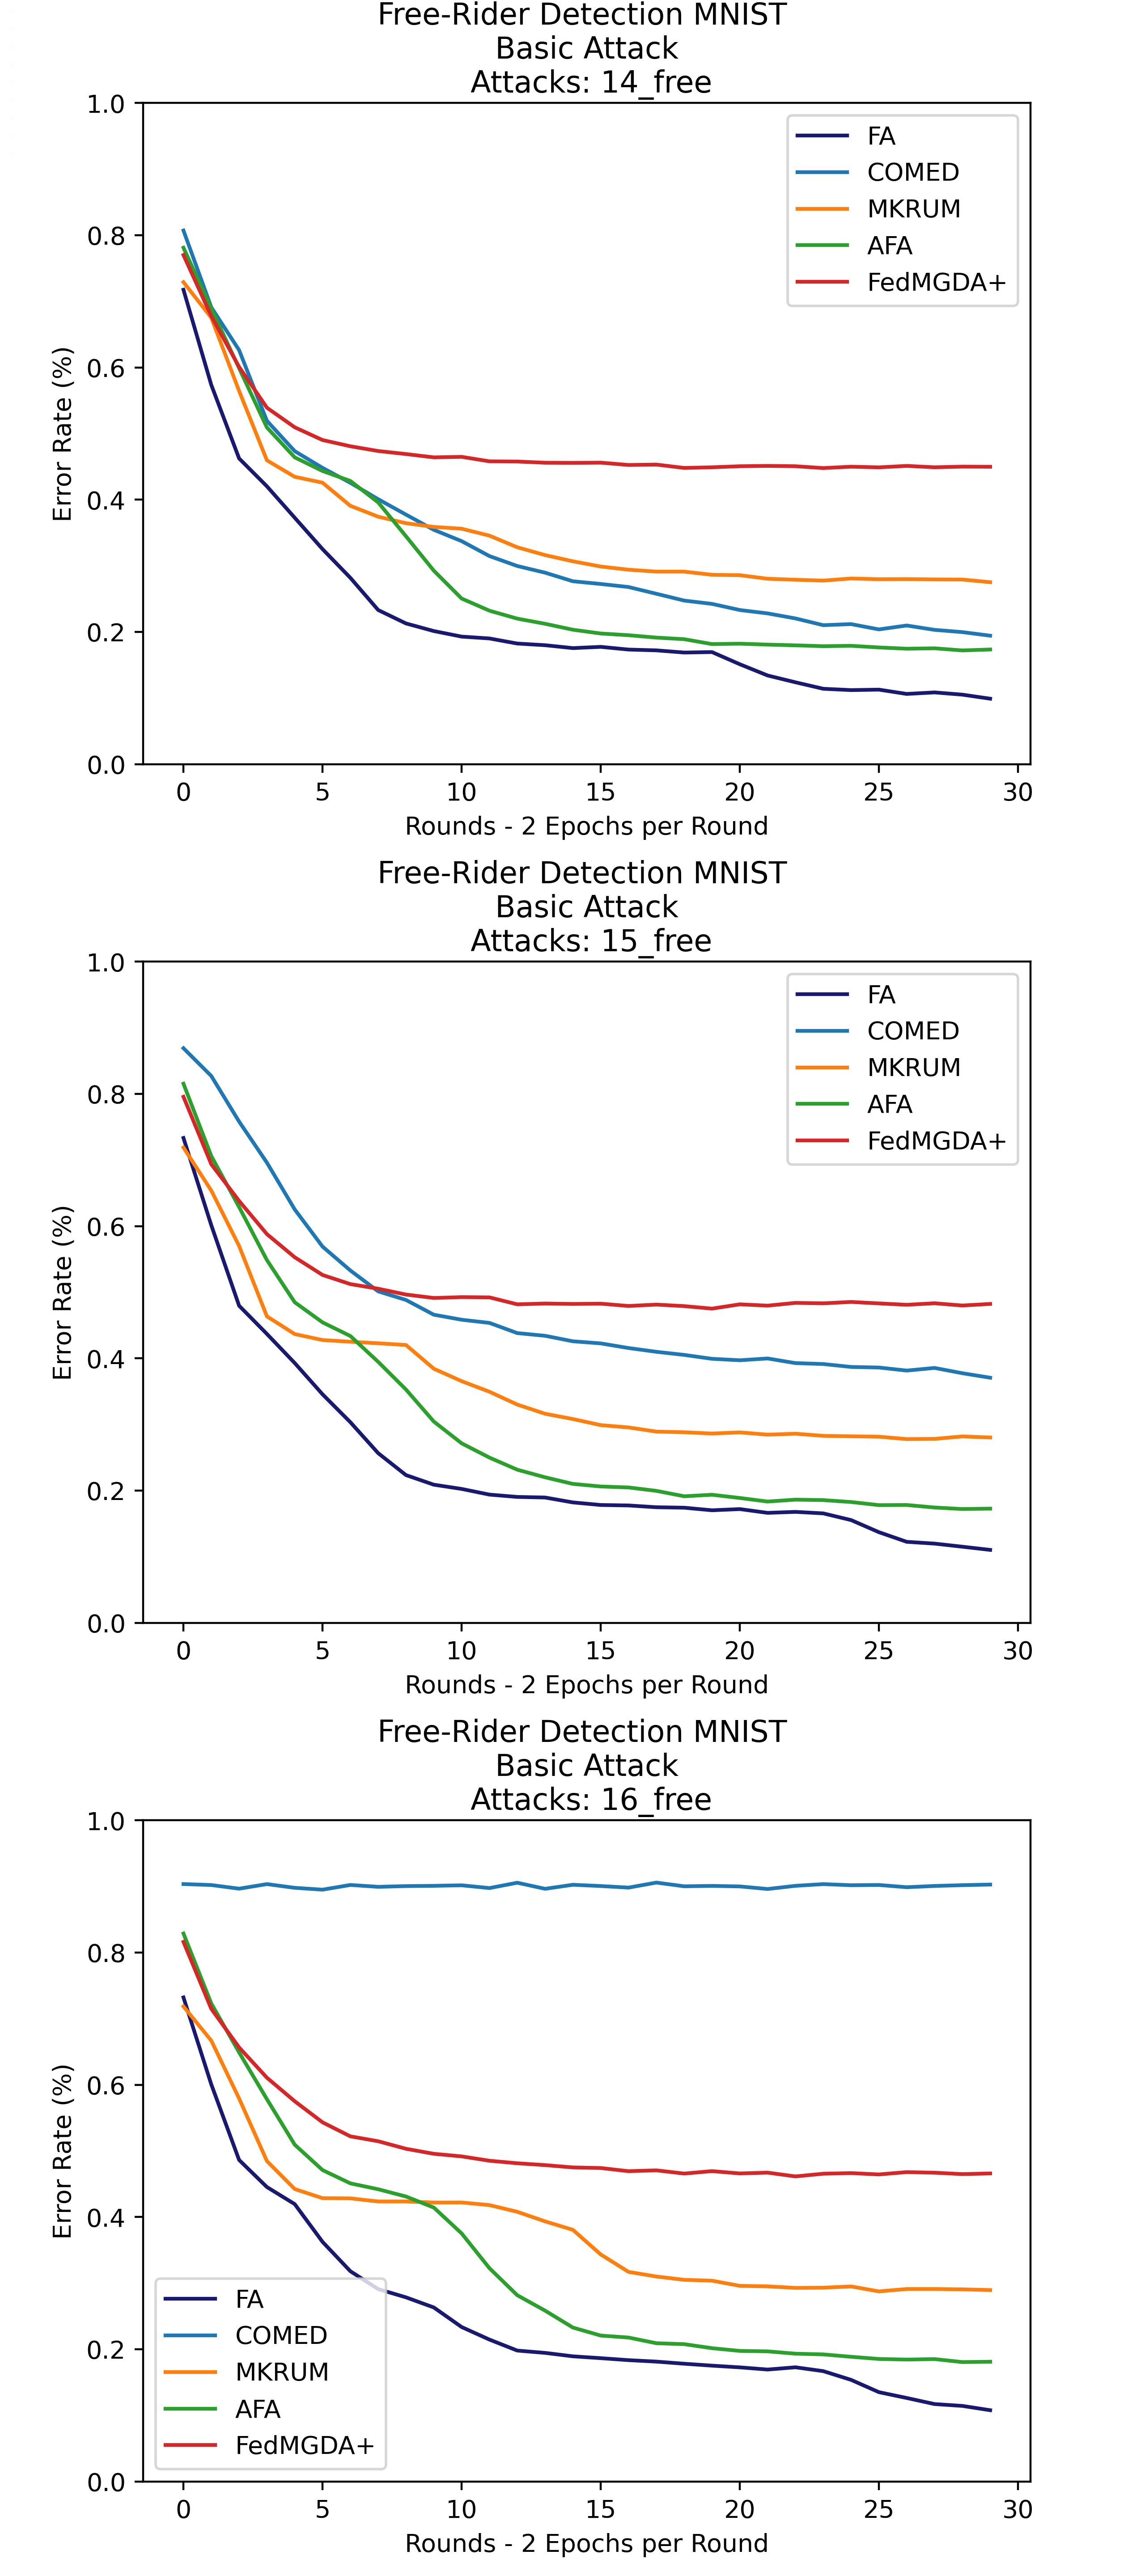
\includegraphics[scale=0.1]{free_riders/graphs/comed_broken.png}
	\caption{Transition of COMED's Error Rate Drastically Increasing as it Breaks the Threshold}
	\label{fig:comed_broken}
\end{figure}

\begin{figure}[htbp]
	\centering
    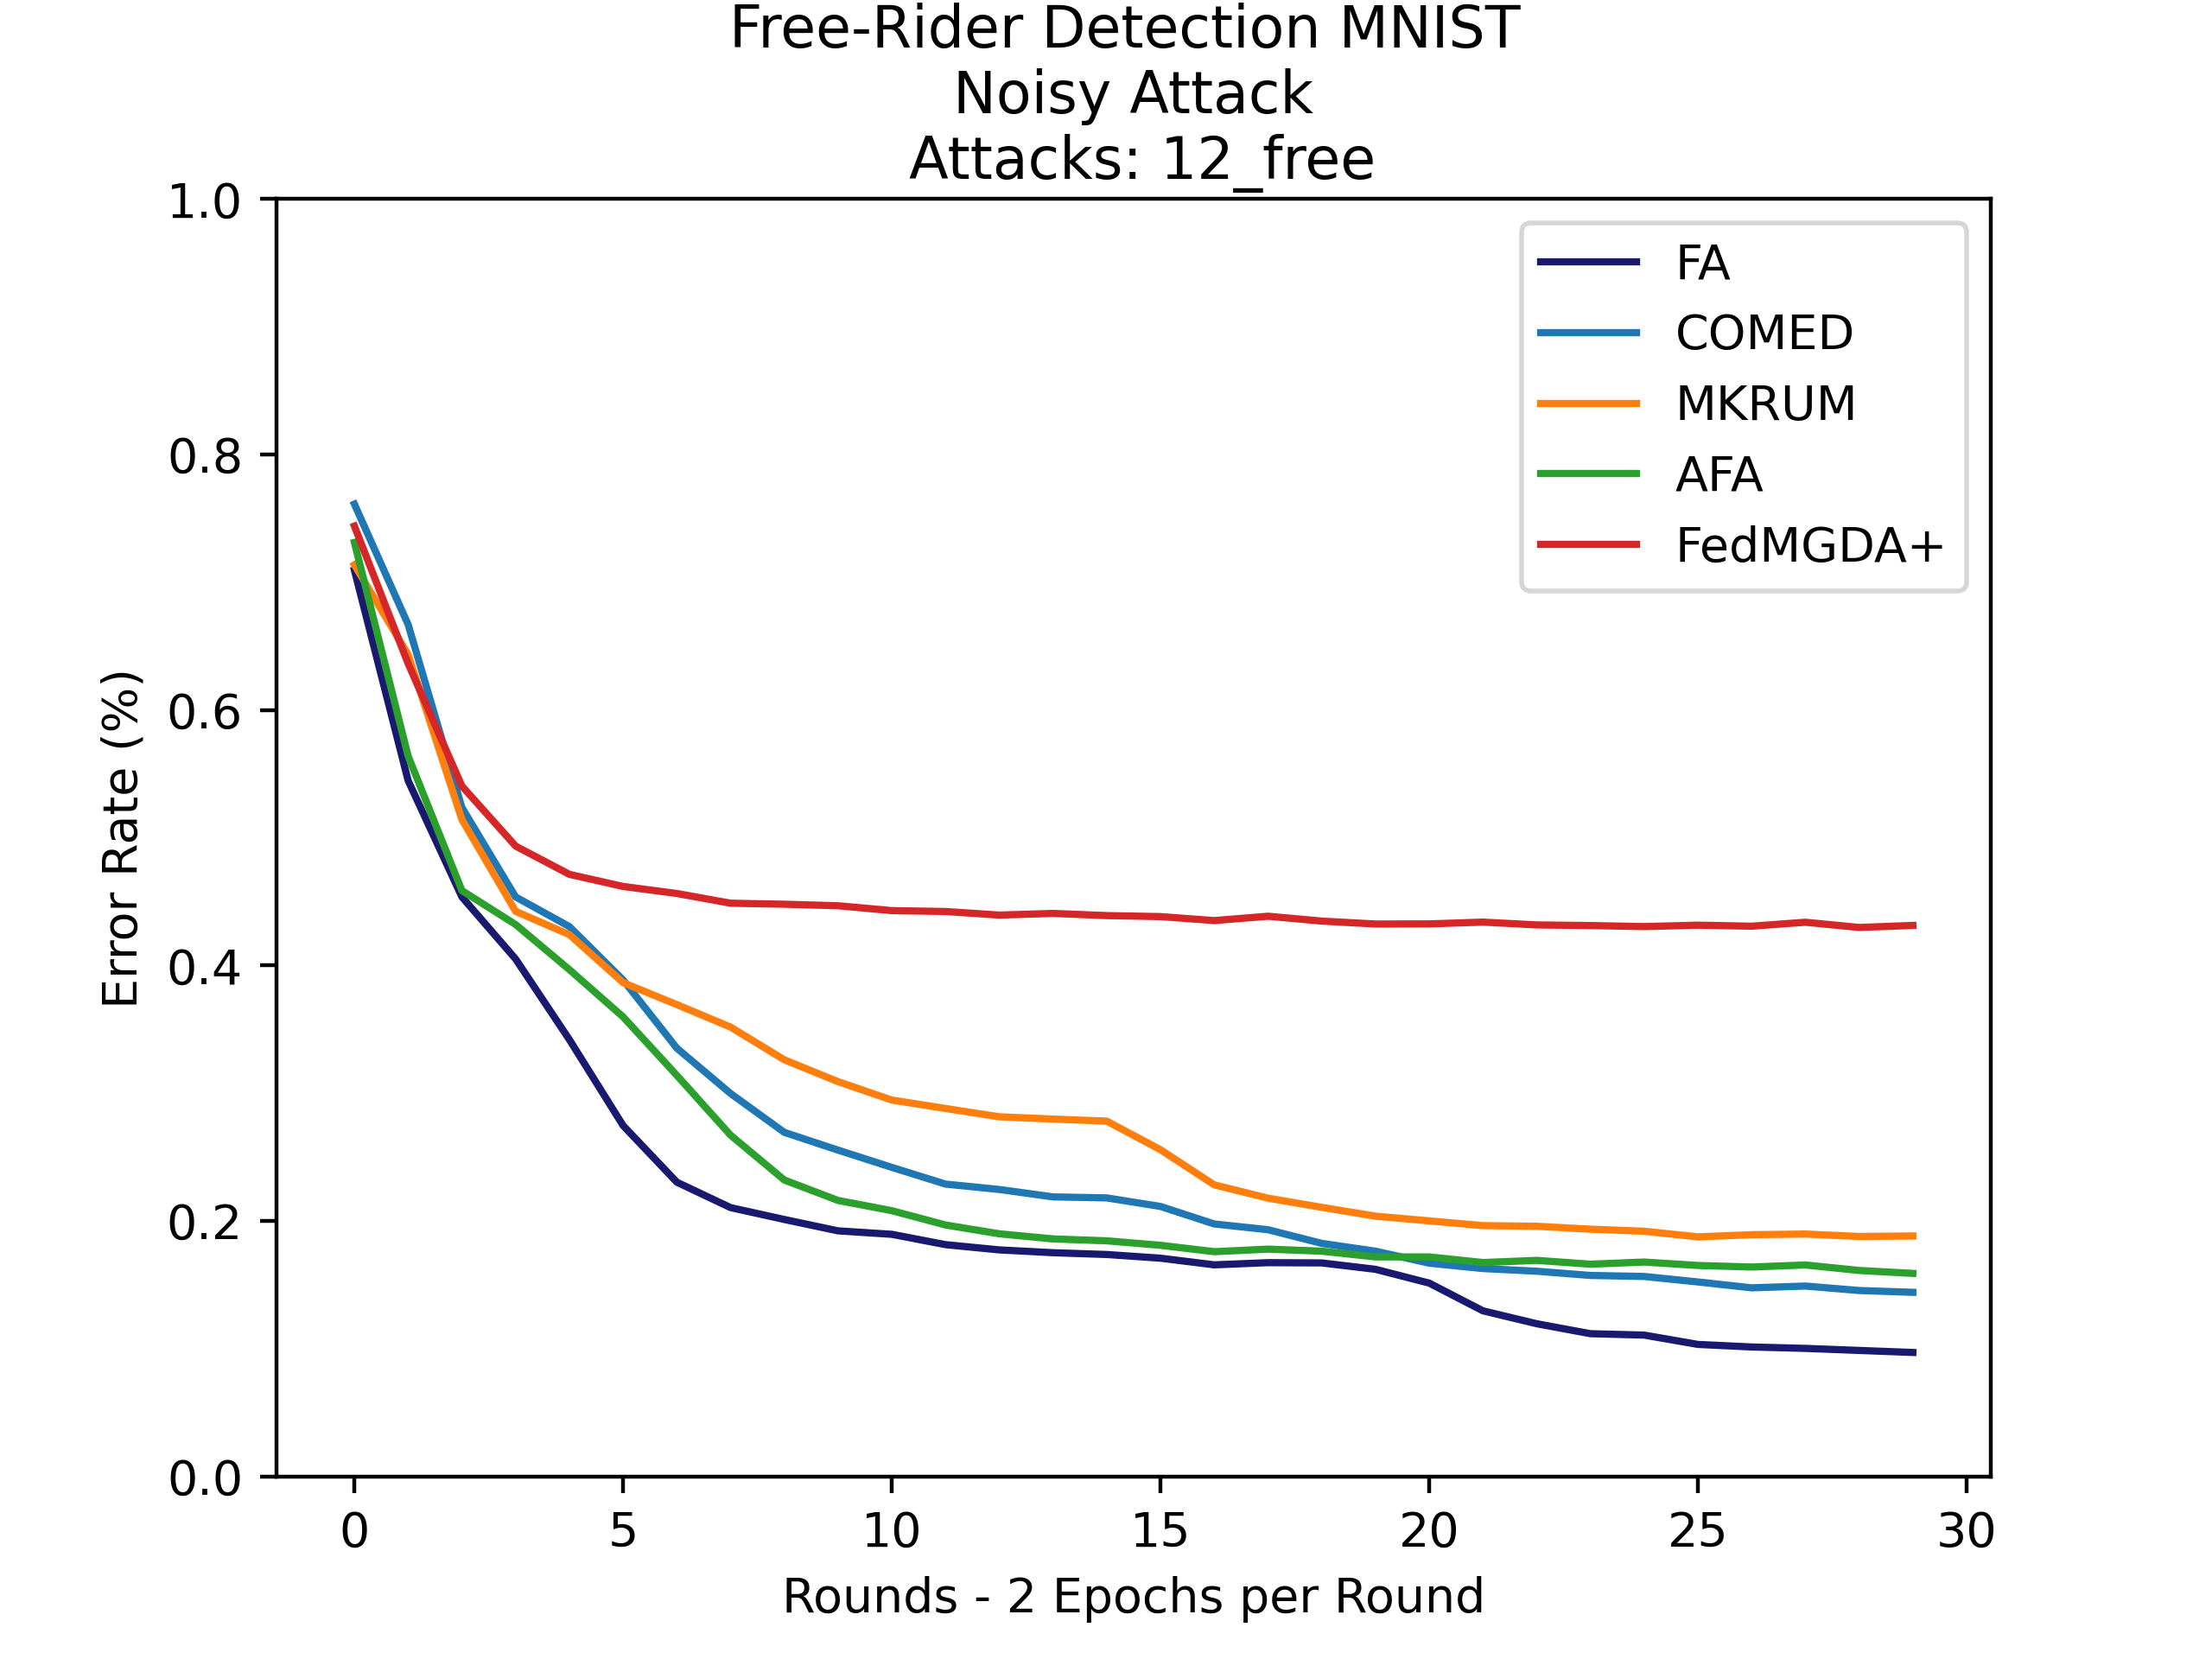
\includegraphics[scale=0.5]{free_riders/graphs/flat_line.png}
	\caption{Error Rate Graph Showing the Flat-Lining of FedMGDA++ once all of the Benign Clients are Blocked}
	\label{fig:flat_line}
\end{figure}